\section{Umsetzung des realen Clusters}\label{sec:aufbauCluster}

\subsection{Hadoop-Benchmark}\label{sec:hadoopBenchmark}

\citeauthor{zhang2016} haben im Rahmen ihrer gesamten Forschungsarbeit die Open"=Source"=Plattform Hadoop-Benchmark entwickelt und auf Github zur Verfügung gestellt.\footnote{\url{https://github.com/Spirals-Team/hadoop-benchmark}} Die Plattform ist in mehrere Szenarien unterteilt, darunter ein Hadoop in der Version 2.7.1 ohne Änderungen und ein darauf basierendes Szenario mit der Selfbalancing-Komponente. Hadoop-Benchmark basiert auf der Software \emph{Docker}\footnote{\url{https://www.docker.com/}} und dem dazugehörigen Tool \emph{Docker Machine}, um damit einfach und schnell ein Hadoop-Cluster aufbauen zu können. Mit \emph{Graphite}\footnote{\url{https://graphiteapp.org/}} ist zudem ein Monitoring-Tool enthalten, mit dem die Performance des Clusters überwacht und analysiert werden kann.

\begin{figure}
    \centering
    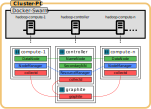
\includegraphics[width=.8\columnwidth]{./images/hadoopBenchmarkArch.png}
    \caption[High-Level-Architektur von Hadoop-Benchmark]{High-Level-Architektur von Hadoop-Benchmark \cite{abb:hadoopBenchmarkArch}}
    \label{fig:hadoopBenchmarkArchitecture}
\end{figure}

Mithilfe von Docker Machine können spezielle Virtuelle Maschinen erstellt werden, die direkt für den Einsatz mit Docker ausgestattet sind. Auf jeder dieser VMs können dadurch direkt ein oder mehrere Docker-Container gestartet werden, welche letztlich das Hadoop-Cluster bilden. Jeder Container enthält, neben dem Hadoop-Controller bzw. -Node, das Tool \emph{collectd}\footnote{\url{https://collectd.org/}}, was das Monitoring des Hadoop-Nodes auf Systemebene übernimmt und die Daten an den Graphite-Container auf der Controller-Machine übermittelt. Es ist dabei möglich, eine beliebige Anzahl an Nodes zu nutzen. Auch ist es möglich, den VMs einen beliebig großen Arbeitsspeicher zur Verfügung zu stellen.

Die Plattform Hadoop-Benchmark enthält auch die bereits in \autoref{sec:lastprofilerstellung} erwähnten Benchmarks Mapreduce Examples, HiBench und SWIM. Sie werden ebenfalls als jeweils eigene Docker-Container gestartet und so an das Cluster übermittelt.

\subsection{Genutztes Cluster in der Fallstudie}\label{sec:clusterFallstudie}

Als reales Hadoop-Cluster für diese Fallstudie soll nun ebenfalls die Plattform Hadoop-Benchmark zum Einsatz kommen. Da Docker und Hadoop vor allem für den Einsatz in einer Linux-Umgebung entwickelt wurden, wird dazu ein eigener PC mit Ubuntu 16.04 LTS genutzt. Da \sS das .NET-Framework, und damit Windows, benötigt, wird dafür ebenfalls ein eigener PC verwendet. Im konkreten Versuchsaufbau wird für Windows eine VM genutzt, welche auf einem anderen PC als das Cluster ausgeführt wird. Die genauen Spezifikationen der PCs und der Windows-VM sind in \autoref{fig:pcSpecs} aufgelistet.

\begin{figure}
    \centering
    \begin{tabular}{|c|c|c|c|}
    	\hline
    	     \textbf{}      & \textbf{Cluster-PC} & \textbf{VM-PC} & \textbf{Windows-VM}  \\ \hline\hline
    	   \textbf{CPU}     &    Intel Core i5    & Intel Core i5  &       2 Cores        \\ \hline
    	   \textbf{RAM}     &        16 GB        &     16 GB      &         6 GB         \\ \hline
    	\textbf{Festplatte} &     500 GB HDD      &   128 GB SSD   &  $\leq$ 100 GB VHD   \\ \hline
    	    \textbf{OS}     &  Ubuntu 16.04 LTS   & Kubuntu 16.10  & Windows 10 1709 Edu. \\ \hline
    \end{tabular}
    \caption{Spezifikationen der verwendeten PCs und Windows-VM}
    \label{fig:pcSpecs}
\end{figure}

Auf dem Cluster-PC nutzt Docker-Machine zur Erstellung, Verwaltung und Ausführung der VMs die Treiber von VirtualBox 5.2\footnote{\url{https://www.virtualbox.org/}}. Für das Cluster werden 4 Nodes, der Controller sowie eine Consul-VM zur internen Verwaltung der Netzwerkverbindungen zwischen den VMs und Docker-Containern erstellt. Jeder der vier Nodes und der Controller erhalten jeweils 2 GB RAM, für den Consul sind 512 MB ausreichend. Für die Windows-VM wird ebenfalls VirtualBox 5.2 eingesetzt.

%TODO: Link zum angepassten Hadoop-Benchmark?
In keinem Szenario der Plattform Hadoop-Benchmark wird standardmäßig der Timeline-Server von Hadoop gestartet. Daher wurde basierend auf dem Selfbalancing-Szenario ein neues Szenario erstellt, bei dem der Timeline-Server gestartet wird. Dadurch ist einerseits die Selfbalancing-Komponente von \citeauthor{zhang2016} aktiv und andererseits besteht die Möglichkeit, für das Monitoring zusätzlich den Timeline-Server zu nutzen.

Um viele standardmäßige Aufgaben und Möglichkeiten zu vereinfachen, wurde zudem ein eigenes Setup-Script erstellt. Es vereinfacht folgende Aufgaben:

\begin{itemize}[noitemsep]
    \item Starten, Beenden und Löschen des kompletten Clusters mit Hadoop
    \item Starten und Beenden des Docker-Containers eines Nodes
    \item Hinzufügen und Entfernen der Netzwerkverbindung des Docker-Containers eines Nodes
    \item Ausführen der verwendeten Benchmarks
    \item Ausführen von eigenen Befehlen auf dem Docker-Container des Controllers
\end{itemize}

Für die Befehle, die das gesamte Cluster betreffen, wird vom Setup-Script meist auf das in Hadoop-Benchmark enthaltene Start-Script zugegriffen. Die Befehle, welche die Docker-Container der Nodes betreffen, sowie das Ausführen von Befehlen im Controller-Container, werden vom Setup-Script direkt ausgeführt. Für das Starten der Benchmarks werden dagegen die in Hadoop-Benchmark enthaltenen Ausführungs-Scripte der Benchmarks gestartet.